%%
%% Automatically generated ptex2tex (extended LaTeX) file
%% from Doconce source
%% http://code.google.com/p/doconce/
%%




%-------------------------- begin preamble --------------------------
\documentclass[twoside]{article}



\usepackage{relsize,epsfig,makeidx,amsmath,amsfonts}
\usepackage[latin1]{inputenc}
\usepackage{minted} % packages needed for verbatim environments


% Hyperlinks in PDF:
\usepackage[%
    colorlinks=true,
    linkcolor=black,
    %linkcolor=blue,
    citecolor=black,
    filecolor=black,
    %filecolor=blue,
    urlcolor=black,
    pdfmenubar=true,
    pdftoolbar=true,
    urlcolor=black,
    %urlcolor=blue,
    bookmarksdepth=3   % Uncomment (and tweak) for PDF bookmarks with more levels than the TOC
            ]{hyperref}
%\hyperbaseurl{}   % hyperlinks are relative to this root

% Tricks for having figures close to where they are defined:
% 1. define less restrictive rules for where to put figures
\setcounter{topnumber}{2}
\setcounter{bottomnumber}{2}
\setcounter{totalnumber}{4}
\renewcommand{\topfraction}{0.85}
\renewcommand{\bottomfraction}{0.85}
\renewcommand{\textfraction}{0.15}
\renewcommand{\floatpagefraction}{0.7}
% 2. ensure all figures are flushed before next section
\usepackage[section]{placeins}
% 3. enable begin{figure}[H] (often leads to ugly pagebreaks)
%\usepackage{float}\restylefloat{figure}

\newcommand{\inlinecomment}[2]{  ({\bf #1}: \emph{#2})  }
%\newcommand{\inlinecomment}[2]{}  % turn off inline comments

% insert custom LaTeX commands...

\makeindex

\begin{document}
%-------------------------- end preamble --------------------------





% ----------------- title -------------------------

\begin{center}
{\LARGE\bf INF5620 Compulsory Project}\\
{\LARGE\bf 2D Wave Equation}
\end{center}




% ----------------- author(s) -------------------------

\begin{center}
{\bf Ingeborg Sauge Torpe (\texttt{ingebto@student.matnat.uio.no})} \\ [0mm]
{\bf Nina Kristine Kylstad (\texttt{ninakky@student.matnat.uio.no})} \\ [0mm]
{\bf Heidi Isabell Denis (\texttt{heidiid@student.matnat.uio.no})} \\ [0mm]
\end{center}

\begin{center}
% List of all institutions:
\centerline{INF5620 - Numerical methods for partial differential equations}
\end{center}
% ----------------- end author(s) -------------------------



% ----------------- date -------------------------


\begin{center}
October 31, 2012
\end{center}

\vspace{1cm}



\begin{abstract}
This report investigates the two dimensional wave equation with variable coefficients.



\end{abstract}

\tableofcontents



% Section with multi-line equation.


\section{Mathematical problem}

\label{math:problem}

\index{model problem} \index{2D wave equation}

We address the standard two-dimensional linear wave equation, with damping,

\begin{align}
\frac{\partial^2 u}{\partial t^2} + b\frac{\partial u}{\partial t} &= \frac{\partial}{\partial x} \left( q(x,y) \frac{\partial u}{\partial x} \right) + \frac{\partial}{\partial y} \left( q(x,y) \frac{\partial u}{\partial y} \right) + f(x,y,t), \label{eq:wave}\\
u(x,y,0)  &= I(x,y),                         \label{initial:values}\\
u_t(x,u,0) &= V(x,y),                         \label{initial:values:t}\\
\frac{\partial u}{\partial n} &= 0,
\end{align}
where $b$, $q$, $I$ and $V$ are prescribed parameters, and $u(x,y,t)$ is
the unknown function to be estimated. The equation will be evaluated on a 
rectangular spatial domain $\left[0, L_x \right] \times \left[0, L_y \right]$.

% Section with single-line equation and a bullet list.


\section{Numerical solution}
\label{numerical:problem}
\index{mesh in time} \index{mesh in space} \index{numerical scheme}
\index{finite difference scheme}

\subsection{The general scheme for computing $u_{i,j}^{n+1}$ at interior spatial mesh points}

By means of centered differences, the first- and second-order derivative with respect to time can be expressed as
\begin{equation*}
\frac{\partial}{\partial t} u(x_i, y_j, t^n) \approx \frac{u_{i,j}^{n+1} - u_{i,j}^{n-1}}{2\Delta t} = [D_{2t} u]_{i,j}^n,
\end{equation*}
and
\begin{equation*}
\frac{\partial^2}{\partial t^2} u(x_i, y_j, t^n) \approx \frac{u_{i,j}^{n+1} - 2u_{i,j}^n + u_{i,j}^{n-1}} {\Delta t^2} = \left[D_t D_t u \right]_{i,j}^n,
\end{equation*}
respectively. 

There are similar discretizations for the first- and second-order derivatives in space. By replacing the derivatives in \eqref{eq:wave} with these finite differences, we get the general scheme for the interior
spatial mesh points:

\begin{align}
u_{i,j}^{n+1} &= (1+\frac{b}{2}\Delta t)^{-1} \bigg[2u_{i,j}^n - (1-\frac{b}{2}\Delta t) u_{i,j}^{n-1} + \Delta t^2 f_{i,j}^n \nonumber \\
&+ \frac{\Delta t^2}{\Delta x^2} \left(q_{i+\frac{1}{2},j} (u_{i+1,j}^n - u_{i,j}^n) -  q_{i-\frac{1}{2},j} (u_{i,j}^n - u_{i-1,j}^n) \right) \\
&+ \frac{\Delta t^2}{\Delta y^2} \left(q_{i,j+\frac{1}{2}} (u_{i,j+1}^n - u_{i,j}^n) -  q_{i,j-\frac{1}{2}} (u_{i,j}^n - u_{i,j-1}^n) \right) \bigg]. \nonumber
\end{align}

The full calculations showing how the scheme was derived can be seen in appendix A.


\subsection{The modified scheme at the boundary points}
\label{boundary:conditions}

Due to the imposed Neumann condition on the boundary,
\begin{equation*}
\frac{\partial u}{\partial n} = \mathbf{n} \cdot \nabla u = n_x\frac{\partial u}{\partial x} + n_y \frac{\partial u}{\partial y} = 0. 
\end{equation*}

On the edge $x=0$ the normal vector pointing out of the spatial domain is $-\hat{i} = (-1,0)$, so consequently $\frac{\partial u}{\partial n} = -\frac{\partial u}{\partial x}$.
Discretizing this for $\{y_j\}_{j=0}^{N_y}$ and $\{t^n\}_{n=0}^N$ provide the relation
\begin{equation}
-\frac{u_{1,j}^n - u_{-1,j}^n}{2\Delta x} = 0 \ \implies u_{-1,j}^n = u_{1,j}^n.
\label{bc:x0}
\end{equation}


On the edge $x=L_x$ the normal vector pointing out of the spatial domain is $\hat{i} = (1,0)$, so consequently $\frac{\partial u}{\partial n} = \frac{\partial u}{\partial x}$.
Discretizing this for $\{y_j\}_{j=0}^{N_y}$ and $\{t^n\}_{n=0}^N$ provide the relation
\begin{equation}
\frac{u_{N_x + 1,j}^n - u_{N_x - 1,j}^n}{2\Delta x} = 0 \ \implies u_{N_x + 1,j}^n = u_{N_x - 1,j}^n.
\label{bc:xL}
\end{equation}


On the edge $y=0$ the normal vector pointing out of the spatial domain is $-\hat{j} = (0,-1)$, so consequently $\frac{\partial u}{\partial n} = -\frac{\partial u}{\partial y}$.
Discretizing this for $\{x_i\}_{i=0}^{N_x}$ and $\{t^n\}_{n=0}^N$ provide the relation
\begin{equation}
-\frac{u_{i,1}^n - u_{i,-1}^n}{2\Delta y} = 0 \ \implies u_{i,-1}^n = u_{i,1}^n.
\label{bc:y0}
\end{equation}


On the edge $y=L_y$ the normal vector pointing out of the spatial domain is $\hat{j} = (0,1)$, so consequently $\frac{\partial u}{\partial n} = \frac{\partial u}{\partial y}$.
Discretizing this for $\{x_i\}_{i=0}^{N_x}$ and $\{t^n\}_{n=0}^N$ provide the relation
\begin{equation}
\frac{u_{i,N_y + 1}^n - u_{i,N_y - 1}^n}{2\Delta y} = 0 \ \implies u_{i,N_y + 1}^n = u_{i,N_y -1}^n.
\label{bc:yL}
\end{equation}

In appendix A, the complete schemes for the points at the boundary are derived. However, ghost points rather than the modified schemes are used in the actual implementation.


\subsection{The modified scheme for the first step at interior points}

The initial conditions \eqref{initial:values} and \eqref{initial:values:t} imply that
\begin{equation}
u_{i,j}^0 = I(x_i, y_j), 
\label{ic}
\end{equation}
and
\begin{equation}
\frac{u_{i,j}^{1} - u_{i,j}^{-1}}{2 \Delta t} = V(x_i,y_j),
\label{ic:t}
\end{equation}
for all  $i=1, ..., N_x - 1$ and $j=1, ..., N_y - 1$.
Now, evaluating the scheme at $t_1$ one may eliminate the contribution from the point outside the mesh, that is
\begin{align*}
u_{i,j}^{1} &= (1+\frac{b}{2}\Delta t)^{-1} \bigg[2u_{i,j}^0 - (1-\frac{b}{2}\Delta t) u_{i,j}^{-1} + \Delta t^2 f_{i,j}^0 \nonumber \\
&+ \frac{\Delta t^2}{\Delta x^2} \left(q_{i+\frac{1}{2},j} (u_{i+\frac{1}{2},j}^0 - u_{i,j}^0) -  q_{i-\frac{1}{2},j} (u_{i,j}^0 - u_{i-\frac{1}{2},j}^0) \right) \\
&+ \frac{\Delta t^2}{\Delta y^2} \left(q_{i,j+\frac{1}{2}} (u_{i,j+\frac{1}{2}}^0 - u_{i,j}^0) -  q_{i,j-\frac{1}{2}} (u_{i,j}^0 - u_{i,j-\frac{1}{2}}^0) \right) \bigg]. \nonumber
\end{align*}
From \eqref{ic:t}, we get the condition $u_{i,j}^{-1} = u_{i,j}^1 - 2\Delta t V_{i,j}$. Inserting this condition into the general scheme provides the scheme for the first step:
\begin{align}
u_{i,j}^1 &= I_{i,j} + \Delta t(1- \frac{b}{2} \Delta t) V_{i,j} + \frac{1}{2} \bigg[\Delta t^2 f_{i,j}^0 \nonumber \\
&+ \frac{\Delta t^2}{\Delta x^2} \left(q_{i+\frac{1}{2},j} (u_{i+\frac{1}{2},j}^0 - u_{i,j}^0) -  q_{i-\frac{1}{2},j} (u_{i,j}^0 - u_{i-\frac{1}{2},j}^0) \right) \\
&+ \frac{\Delta t^2}{\Delta y^2} \left(q_{i,j+\frac{1}{2}} (u_{i,j+\frac{1}{2}}^0 - u_{i,j}^0) -  q_{i,j-\frac{1}{2}} (u_{i,j}^0 - u_{i,j-\frac{1}{2}}^0) \right) \bigg]. \nonumber
\end{align}

\subsection{The modified scheme for the first step at boundary points}

Here, we can use the same conditions that were derived in section \ref{boundary:conditions}. Again is is most convenient to use ghost points in the actual implementation.

\noindent


\section{Implementation}

The numerical scheme derived above is implemented in the program $wave\_solver.py$, which can be found in appendix B. A sample of the function used to implement the general scheme for all mesh points after the first step (using ghost points) is shown below. This is a vectorized function.

\begin{minted}[fontsize=\fontsize{9pt}{9pt},linenos=false,mathescape,baselinestretch=1.0,fontfamily=tt,xleftmargin=7mm]{python}
def advance_vectorized(X, Y ,u, u_1, u_2, q, f, c1, c2, Cx2, Cy2, dt2, tn, b, dx, w, \
		Nx, Ny, exact):
    # boundary conditions using ghost points:
    u_1[0,:] = u_1[2,:] # u[-1, y] = u[1, y]
    u_1[-1,:] = u_1[-3,:] # u[Nx+1, y] = u[Nx-1, y]
    u_1[:,0] = u_1[:,2] # u[x, -1] = u[x, 1]
    u_1[:,-1] = u_1[:,-3] # u[x, Ny+1] = u[x, Ny-1]
    
    # Scheme for all interior points
    u[1:-1,1:-1] = c1*(2*u_1[1:-1,1:-1] - c2*u_2[1:-1,1:-1] + \
      0.5*Cx2*((q[1:-1,1:-1] + q[2:,1:-1])*(u_1[2:,1:-1]-u_1[1:-1,1:-1]) - \
      (q[1:-1,1:-1] + q[:-2,1:-1])*(u_1[1:-1,1:-1] - u_1[:-2,1:-1])) + \
      0.5*Cy2*((q[1:-1,1:-1] + q[1:-1,2:])*(u_1[1:-1,2:] - u_1[1:-1,1:-1]) - \
      (q[1:-1,1:-1] + q[1:-1,:-2])*(u_1[1:-1,1:-1] - u_1[1:-1,:-2])) + dt2*f[1:-1,1:-1])
      
    if exact is not None:
        # Compare numerical soluion with exact solution
        Err = exact[1:-1,1:-1] - u[1:-1,1:-1]  
        E = sqrt(dx*dx*sum(Err**2))
    else:
        E = 0
    
    u_2 = u_1.copy()
    u_1 = u.copy()
    return u_1, u_2, E
\end{minted}

% Section with figures.


\section{Verification}
\index{verification}

\subsection{Constant solution}
\index{constant solution}

A test case is constructed with $u = 1.2$ as a solution. This constant is returned by the solver for both the vectorized and scalar versions:

\begin{minted}[fontsize=\fontsize{9pt}{9pt},linenos=false,mathescape,baselinestretch=1.0,fontfamily=tt,xleftmargin=7mm]{python}
$ python test_constant.py 
Scalar:
dx:  0.2
dy:  0.2
[[ 1.2  1.2  1.2 ...,  1.2  1.2  1.2]
 [ 1.2  1.2  1.2 ...,  1.2  1.2  1.2]
 [ 1.2  1.2  1.2 ...,  1.2  1.2  1.2]
 ..., 
 [ 1.2  1.2  1.2 ...,  1.2  1.2  1.2]
 [ 1.2  1.2  1.2 ...,  1.2  1.2  1.2]
 [ 1.2  1.2  1.2 ...,  1.2  1.2  1.2]]
Vectorized:
dx:  0.2
dy:  0.2
[[ 1.2  1.2  1.2 ...,  1.2  1.2  1.2]
 [ 1.2  1.2  1.2 ...,  1.2  1.2  1.2]
 [ 1.2  1.2  1.2 ...,  1.2  1.2  1.2]
 ..., 
 [ 1.2  1.2  1.2 ...,  1.2  1.2  1.2]
 [ 1.2  1.2  1.2 ...,  1.2  1.2  1.2]
 [ 1.2  1.2  1.2 ...,  1.2  1.2  1.2]]
\end{minted}

The program can be found in appendix \ref{test:constant:py}


\subsection{Exact 1D solution}
\index{1D solution}


A simple 1D square or plug wave, $I(x,y)=2$ for x less than some value and $I=0$ otherwise should when $\frac{c\Delta t}{\Delta x} = 1$ propagate with exact plug shape and amplitude 1 through the domain for any $\Delta y$. This verification simulates an exact discrete solution of the 1D wave equation in a 2D program. 

The implementation of the plug can be seen in appendix \ref{test:1D:plug:py}. The results can be seen in the figure below:

\begin{center}  % inline figure
  \centerline{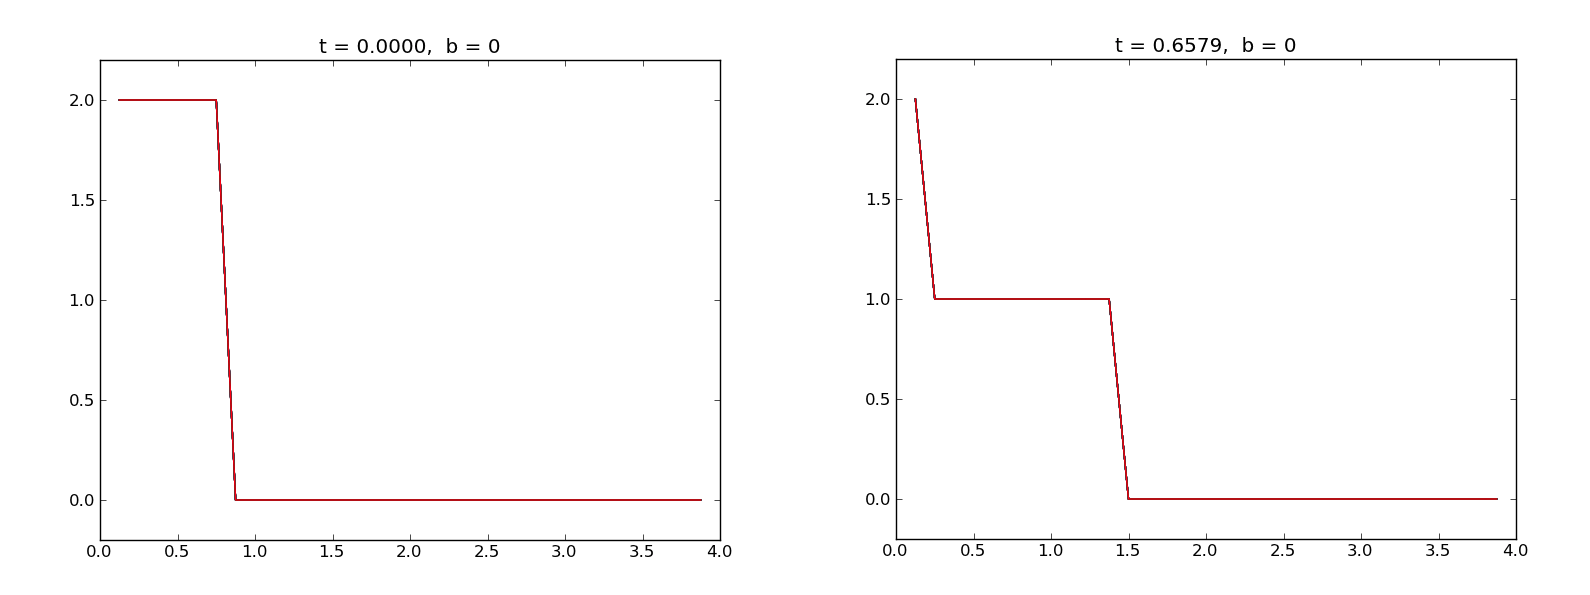
\includegraphics[width=0.9\linewidth]{1Dpluga.png}}
  \centerline{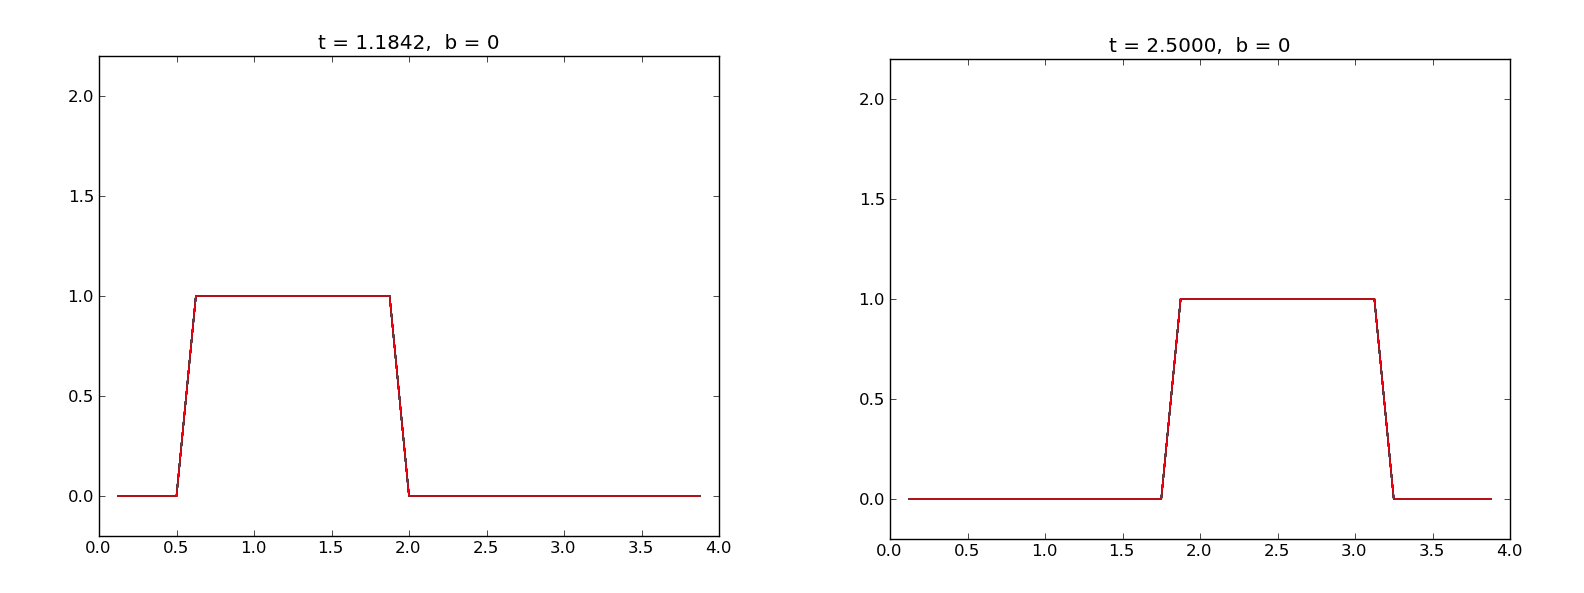
\includegraphics[width=0.9\linewidth]{1Dplugb.png}}
\end{center}


\subsection{Standing wave}

The program was tested with a manufactured solution. With constant q, the exact solution used was:
\begin{equation}
u(x,y,t)=exp(-bt)cos(m_xx\pi/Lx)cos(m_yy\pi/Ly)cos(\omega t)
\label{standing:wave:exact}
\end{equation}
for arbitrary integers $m_x$ and $m_y$ and a suitable choice of $\omega$. The boundary conditions that were used are the same as earlier, so the solution is a standing wave with $\frac{\partial u}{\partial n} = 0$.
Expressions for $I(x,y)$, $V(x,y)$ and $f(x,y)$ were derived from \eqref{standing:wave:exact}.

Since the given u is not an exact solution of the discrete equations, the test must be based on empirical analysis of the convergence. The error E is assumed to behave like
\begin{equation}
E=C_t\Delta t^2+C_x\Delta x^2+C_y\Delta y^2,
\end{equation}
for some constants $C_t$, $C_x$, and $C_y$. We choose $\Delta t=F_th$, $\Delta x=F_xh$ and $\Delta y=F_yh$ where $h$ is a common discretization parameter to be varied ($h\rightarrow 0$) and $F_t$, $F_x$, and $F_y$ are freely chosen constant factors compatible with the stability criterion in 2D. The error can then be expressed as
\begin{equation}
E=Ch^2
\end{equation}
where $C=C_xF^2_t+C_yF^2_x+C_tF^2_t.$

Experiments were performed with decreasing $h$, and the error $E$ was computed. A convergence test was also run on the error. The results were as follows:

\begin{verbatim}
$ python test_standing_wave.py vectorized
dx:  0.2
dy:  0.2
dx:  0.1
dy:  0.1
dx:  0.05
dy:  0.05
dx:  0.025
dy:  0.025
dx-list:
[0.2, 0.1, 0.05, 0.025]
E/dx**2: 
[11.756040451767683, 12.201635681383843, 12.633992353221144, 12.995352031196109]
Convergence rates: 
[1.9463276681446646, 1.9497639560514375, 1.9593148886166989]
\end{verbatim}

From these results, it can be seen that $E/h^2$ is approximately constant (although it is increasing slightly for smaller $h$). The convergence test appears to show convergence towards $2$, although the values are still \emph{slightly} smaller than expected. Perhaps there is still a bug somewhere in the program. The source code for the program can be found in appendix \ref{test:standing:wave:py}.

\subsection{Manufactured solution}

A similar analysis was done as in the previous section. This time, $q(x,y)$ was not a constant but rather a function varying with $x$ and $y$.

\begin{verbatim}
$ python test_manufactured_solution.py vectorized
dx:  0.2
dy:  0.2
dx:  0.1
dy:  0.1
dx:  0.05
dy:  0.05
dx:  0.025
dy:  0.025
dx-list:
[0.2, 0.1, 0.05, 0.025]
E/dx**2: 
[366.58399859657737, 679.95269048763794, 1308.7523812765949, 2571.3684952980771]
Error_list:
[14.663359943863098, 6.7995269048763811, 3.2718809531914879, 1.6071053095612984]
Convergence rates: 
[1.1087094430469164, 1.0553141134886745, 1.0256557887500868]
\end{verbatim}

Here, the convergence rate appears to be $1$. This definitely points to some (well hidden) bug in the program.
On the bright side, the convergence rate for the scalar version seems to be approximately the same as for the vectorized version:
\begin{verbatim}
$ python test_manufactured_solution.py scalar
dx:  0.2
dy:  0.2
dx:  0.1
dy:  0.1
dx:  0.05
dy:  0.05
dx-list:
[0.2, 0.1, 0.05]
E/dx**2: 
[396.37377651332247, 725.59881374267093, 1360.446884531819]
Error_list:
[15.854951060532903, 7.2559881374267103, 3.4011172113295483]
Convergence rates: 
[1.1276894219158444, 1.093163371334972]
\end{verbatim}

The source code for the program used can be found in appendix \ref{test:man:solution:py}.


\section{Extension - 3D visualisation using Mayavi}

For the extension, a simple Gaussian wave was used. $q(x,y)$ was set up such that it represented a simple Gaussian underwater mountain. To see what would happen, $q(x,y)$ was also set up to represent a simple (plane) underwater slope. The program for this can be found in appendix \ref{run:gaussian:py}.

For each time step, the matrix containing the values of $u(x,y,t)$ was saved to a file. Each file was later read by a plotting script, which created plots of $u$ for each time step, and saved the plot. When all the plots were created and saved, they were collected together to form a movie. 

The source code for the plotting script can be found in appendix \ref{plot:3D:py}.

The movies that were created can be found in the files $Gauss\_wave\_gauss\_hill.gif$ and $tsunami.gif$ respectively. A sample image of each is shown below:

\subsection{Simple Gaussian underwater mountain}
\begin{center}  % inline figure
  \centerline{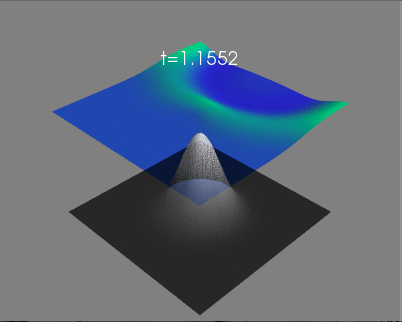
\includegraphics[width=0.8\linewidth]{gauss.png}}
\end{center}

\subsection{Plane underwater slope}
\begin{center}  % inline figure
  \centerline{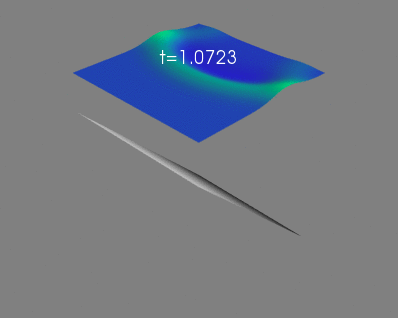
\includegraphics[width=0.8\linewidth]{tsunami.png}}
\end{center}



\appendix
\section{Calculations for the discretization}
\label{app:A}
\subsection{Discretizing the equation}
Let the temporal domain $\left[0, T\right]$ be represented by a finite number of mesh points $\{t^n\}_{n=0}^N$, where
\begin{equation*}
t^0 = 0 < t^1< t^2 < ... < t^{N-1} < tN = T.
\end{equation*}
Similarly, the spatial domains $\left[0,L_x \right]$ and $\left[0,L_y \right]$ are replaced by  $\{x_i\}_{i=0}^{N_x}$ and $\{y_j\}_{j=0}^{N_y}$, respectively, where
\begin{align*}
0 &= x_0 < x_1 < x_2 < ... < x_{N_x - 1} < x_{N_x} = L_x, \\
0 &= y_0 < y_1 < y_2 < ... < y_{N_y - 1} < y_{N_y} = L_y.
\end{align*}
For uniformly distributed mesh points, the constant mesh spacings $\Delta t$, $\Delta x$, and $\Delta y$ may be introduced, such that
\begin{align*}
t^n &= n \Delta t, \qquad n = 0, ..., N, \\
x_i &= i \Delta x, \qquad i = 0, ..., N_x, \\
y_j &= j \Delta y, \qquad j = 0, ..., N_y.
\end{align*}
The solution $u(x,y,t)$ is sought at the mesh points, that is $u(x_i, y_j, t^n)$ for $i = 0, ..., N_x$, $j = 0, ..., N_y$, and $n = 0, ..., N$. The numerical approximation at the mesh point $(x_i, y_j, t^n)$ is denoted by $u_{i,j}^n$.
For a numerical solution by the finite difference method, the condition that (\ref{eq:wave}) holds for all points in the domain $(0, L_x) \times (0, L_y) \times (0, T]$ is therefore reduced to the requirement that the PDE is fulfilled at the mesh points.

By means of centered differences, the first- and second-order derivative with respect to time can be expressed as
\begin{equation*}
\frac{\partial}{\partial t} u(x_i, y_j, t^n) \approx \frac{u_{i,j}^{n+1} - u_{i,j}^{n-1}}{2\Delta t} = [D_{2t} u]_{i,j}^n,
\end{equation*}
and
\begin{equation*}
\frac{\partial^2}{\partial t^2} u(x_i, y_j, t^n) \approx \frac{u_{i,j}^{n+1} - 2u_{i,j}^n + u_{i,j}^{n-1}} {\Delta t^2} = \left[D_t D_t u \right]_{i,j}^n,
\end{equation*}
respectively. Furthermore, the principal idea when discretizing a variable coefficient is to first discretize the outer derivative by means of the centered derivative, and thereafter similarly discretize the inner derivative.
Defining $\phi_x = q(x,y) \frac{\partial u}{\partial x}$, $\phi_y = q(x,y) \frac{\partial u}{\partial y}$, and following through with the above-mentioned description,
\begin{equation*}
\left[\frac{\partial \phi_x}{\partial x} \right]_{i,j}^n \approx \frac{(\phi_x)_{i + \frac{1}{2}, j}^n - (\phi_x)_{i-\frac{1}{2}, j}^n}{\Delta x} = [D_x \phi_x]_{i,j}^n.
\end{equation*}
The contributions from the inner derivative are thus
\begin{equation*}
(\phi_x)_{i + \frac{1}{2}, j}^n = q_{i + \frac{1}{2}, j} \left[\frac{\partial u}{\partial x} \right]_{i + \frac{1}{2}, j}^n \approx q_{i + \frac{1}{2}, j} \frac{u_{i + 1, j}^n - u_{i,j}^n}{\Delta x} = [qD_x u]_{i + \frac{1}{2}, j}^n,
\end{equation*}
and
\begin{equation*}
(\phi_x)_{i - \frac{1}{2}, j}^n = q_{i - \frac{1}{2}, j} \left[\frac{\partial u}{\partial x} \right]_{i - \frac{1}{2}, j}^n \approx q_{i - \frac{1}{2}, j} \frac{u_{i , j}^n - u_{i-1,j}^n}{\Delta x} = [qD_x u]_{i - \frac{1}{2}, j}^n.
\end{equation*}
These intermediate results combined yield that
\begin{equation*}
\left[ \frac{\partial}{\partial x} \left (q(x,y) \frac{\partial u}{\partial x} \right) \right]_{i,j}^n \approx \frac{1}{\Delta x^2} \left(q_{i+\frac{1}{2}, j} (u_{i+1,j}^n - u_{i,j}^n) - q_{i-\frac{1}{2}, j}(u_{i,j}^n - u_{i-1,j}^n) \right)
= \left[D_x q D_x u \right]_{i,j}^n.
\end{equation*}

Similar reasoning may be applied to $\phi_y$, such that
\begin{equation*}
\left[ \frac{\partial}{\partial y} \left (q(x,y) \frac{\partial u}{\partial y} \right) \right]_{i,j}^n \approx \frac{1}{\Delta y^2} \left(q_{i, j+ \frac{1}{2}} (u_{i,j+1}^n - u_{i,j}^n) - q_{i, j-\frac{1}{2}}(u_{i,j}^n - u_{i,j-1}^n) \right)
= \left[D_y q D_y u \right]_{i,j}^n.
\end{equation*}

Hence, a discretization of (\ref{eq:wave}) in terms of centered differences reads
\begin{equation*}
\left[D_t D_t u + b D_{2t} u = c^2(D_x D_x u + D_y D_y u) + f \right]_{i,j}^n.
\end{equation*}
Written out in full detail, this is equivalent to
\begin{align*}
&\frac{u_{i,j}^{n+1} - 2u_{i,j}^n + u_{i,j}^{n-1}} {\Delta t^2} + b\frac{u_{i,j}^{n+1} - u_{i,j}^{n-1}}{2\Delta t} \\
&= \frac{1}{\Delta x^2} \left(q_{i+\frac{1}{2}, j} (u_{i+1,j}^n - u_{i,j}^n) - q_{i-\frac{1}{2}, j}(u_{i,j}^n - u_{i-1,j}^n) \right) \\
&+ \frac{1}{\Delta y^2} \left(q_{i, j+ \frac{1}{2}} (u_{i,j+1}^n - u_{i,j}^n) - q_{i, j-\frac{1}{2}}(u_{i,j}^n - u_{i,j-1}^n) \right) + f_{i,j}^n.
\end{align*}
Due to the arithmetic mean, values for $q$ may be determined even though the function might be discrete, that is
\begin{align*}
q_{i+\frac{1}{2}, j} &= \frac{q_{i,j} + q_{i+1,j}}{2}, \\
q_{i-\frac{1}{2}, j} &= \frac{q_{i,j} + q_{i-1,j}}{2}, \\
q_{i,j+\frac{1}{2}} &= \frac{q_{i,j} + q_{i,j+1}}{2}, \\
q_{i,j-\frac{1}{2}} &= \frac{q_{i,j} + q_{i,j-1}}{2}.
\end{align*} 
Finally, solving for the unknown $u_{i,j}^{n+1}$ result in the scheme
\begin{align}
u_{i,j}^{n+1} &= (1+\frac{b}{2}\Delta t)^{-1} \bigg[2u_{i,j}^n - (1-\frac{b}{2}\Delta t) u_{i,j}^{n-1} + \Delta t^2 f_{i,j}^n \nonumber \\
&+ \frac{\Delta t^2}{\Delta x^2} \left(q_{i+\frac{1}{2},j} (u_{i+1,j}^n - u_{i,j}^n) -  q_{i-\frac{1}{2},j} (u_{i,j}^n - u_{i-1,j}^n) \right) \\
&+ \frac{\Delta t^2}{\Delta y^2} \left(q_{i,j+\frac{1}{2}} (u_{i,j+1}^n - u_{i,j}^n) -  q_{i,j-\frac{1}{2}} (u_{i,j}^n - u_{i,j-1}^n) \right) \bigg]. \nonumber
\end{align}

\subsection{Boundary conditions}

Inserting the condition  \eqref{bc:x0} into the scheme provide a modified scheme for the boundary points at $x=0$, that is
\begin{align}
u_{0,j}^{n+1} &= (1+\frac{b}{2}\Delta t)^{-1} \bigg[2u_{0,j}^n - (1-\frac{b}{2}\Delta t) u_{0,j}^{n-1} + \Delta t^2 f_{0,j}^n \nonumber \\
&+ \frac{\Delta t^2}{\Delta x^2} \left(q_{\frac{1}{2},j} (u_{1,j}^n - u_{0,j}^n) -  q_{-\frac{1}{2},j} (u_{0,j}^n - u_{1,j}^n) \right) \\
&+ \frac{\Delta t^2}{\Delta y^2} \left(q_{0,j+\frac{1}{2}} (u_{0,j+1}^n - u_{0,j}^n) -  q_{0,j-\frac{1}{2}} (u_{0,j}^n - u_{0,j-1}^n) \right) \bigg]. \nonumber
\end{align}

Inserting the condition \eqref{bc:xL} into the scheme provide a modified scheme for the boundary points at $x=L_x$, that is
\begin{align}
u_{N_x,j}^{n+1} &= (1+\frac{b}{2}\Delta t)^{-1} \bigg[2u_{N_x,j}^n - (1-\frac{b}{2}\Delta t) u_{N_x,j}^{n-1} + \Delta t^2 f_{N_x,j}^n \nonumber \\
&+ \frac{\Delta t^2}{\Delta x^2} \left(q_{N_x+\frac{1}{2},j} (u_{N_x-1,j}^n - u_{N_x,j}^n) -  q_{N_x-\frac{1}{2},j} (u_{N_x,j}^n - u_{N_x-1,j}^n) \right) \\
&+ \frac{\Delta t^2}{\Delta y^2} \left(q_{N_x,j+\frac{1}{2}} (u_{N_x,j+1}^n - u_{N_x,j}^n) -  q_{N_x,j-\frac{1}{2}} (u_{N_x,j}^n - u_{N_x,j-1}^n) \right) \bigg]. \nonumber
\end{align}

Inserting the condition \eqref{bc:y0} into the scheme provide a modified scheme for the boundary points at $y=0$, that is
\begin{align}
u_{i,0}^{n+1} &= (1+\frac{b}{2}\Delta t)^{-1} \bigg[2u_{i,0}^n - (1-\frac{b}{2}\Delta t) u_{i,0}^{n-1} + \Delta t^2 f_{i,0}^n \nonumber \\
&+ \frac{\Delta t^2}{\Delta x^2} \left(q_{i+\frac{1}{2},0} (u_{i+1,0}^n - u_{i,0}^n) -  q_{i-\frac{1}{2},0} (u_{i,0}^n - u_{i-1,0}^n) \right) \\
&+ \frac{\Delta t^2}{\Delta y^2} \left(q_{i,\frac{1}{2}} (u_{i,1}^n - u_{i,0}^n) -  q_{i,-\frac{1}{2}} (u_{i,0}^n - u_{i,1}^n) \right) \bigg]. \nonumber
\end{align}

Inserting the condition \eqref{bc:yL} into the scheme provide a modified scheme for the boundary points at $y=L_y$, that is
\begin{align}
u_{i,N_y}^{n+1} &= (1+\frac{b}{2}\Delta t)^{-1} \bigg[2u_{i,N_y}^n - (1-\frac{b}{2}\Delta t) u_{i,N_y}^{n-1} + \Delta t^2 f_{i,N_y}^n \nonumber \\
&+ \frac{\Delta t^2}{\Delta x^2} \left(q_{i+\frac{1}{2},N_y} (u_{i+1,N_y}^n - u_{i,N_y}^n) -  q_{i-\frac{1}{2},N_y} (u_{i,N_y}^n - u_{i-1,N_y}^n) \right) \\
&+ \frac{\Delta t^2}{\Delta y^2} \left(q_{i,N_y+\frac{1}{2}} (u_{i,N_y-1}^n - u_{i,N_y}^n) -  q_{i,N_y-\frac{1}{2}} (u_{i,N_y}^n - u_{i,N_y-1}^n) \right) \bigg]. \nonumber
\end{align}


\section{Source code}
\label{source:code}
\subsection{$wave\_solver.py$}
\label{wave:solver:py}

\begin{minted}[fontsize=\fontsize{9pt}{9pt},linenos=false,mathescape,baselinestretch=1.0,fontfamily=tt,xleftmargin=7mm]{python}
from numpy import *
import math, os, subprocess, sys, glob
from plot_u import plot_u, make_movie

def solver(Lx, Ly, Nx, Ny, T, dt, c, I, q, V, f, b, version, B=None, w=None, exact=None, \
		oneD=False, make_plot=True):
    
    dx_x = linspace(0, Lx, Nx+1)
    dy_y = linspace(0, Ly, Ny+1)

    if version == "scalar":
        x = linspace(0, Lx, Nx+1)
        y = linspace(0, Ly, Ny+1)
    else:
        x = linspace(0, Lx, Nx+3)
        y = linspace(0, Ly, Ny+3)
    X,Y = meshgrid(x,y)     # Create spatial points
    dx = float(dx_x[1] - dx_x[0])   # Calculate dx
    dy = float(dy_y[1] - dy_y[0])   # Calculate dy

    q = q(X,Y)
    q_max = amax(q)

    if make_plot:
        if B:
            B = B(X,Y)
            if version == "scalar":
                savetxt("hill.txt", B)
            else:
                savetxt("hill.txt", B[1:-1,1:-1])

   # optimal value for dt
    stability_limit = (1/float(sqrt(q_max)))*(1/sqrt(1/dx**2 + 1/dy**2))  
    if dt <= 0:
        dt = 1*stability_limit
    elif dt > stability_limit:
        print "Error: dt too large."

    if oneD:    # Special case for 1D
        y = y*0
        dy = 1
        dt = dx/c
        Y,Y = meshgrid(y,y)

    N = int(round(float(T/dt)))
    t = linspace(0,T,N+1)
    c1 = 1/(1 + (b*dt)/2)  # Set constants / help variables to be used in the scheme:
    c2 = 1 - (b*dt)/2
    Cx2 = (dt/dx)**2
    Cy2 = (dt/dy)**2
    dt2 = dt**2
    
    if oneD:
        Cy2 = 0  # Special case for 1D
        
    if make_plot:    
        file = open("initial.txt",'w')
        file.write("Nx="+str(Nx)+"\n")
        file.write("Lx="+str(Lx)+"\n")
        file.write("Ny="+str(Ny)+"\n")
        file.write("Ly="+str(Ly)+"\n")
        file.write("T="+str(T)+"\n")
        file.write("N="+str(N)+"\n")
        file.close()
    
    if version == "scalar":
        u = zeros((Nx+1, Ny+1))  # The new soluion at the next timestep
        u_1 = zeros((Nx+1, Ny+1)) # The solution from the current time step
        u_2 = zeros((Nx+1, Ny+1))  # The solution from the previous time step
    else:
        u = zeros((Nx+3, Ny+3))  # The new soluion at the next timestep
        u_1 = zeros((Nx+3, Ny+3)) # The solution from the current time step
        u_2 = zeros((Nx+3, Ny+3))  # The solution from the previous time step
    
    # Initial conditions
    if version == "scalar":
        for i in range(0,Nx+1):
            for j in range(0,Ny+1):
                u_2[i,j] = I(x[i],y[j])
    else:  # vectorized version
        u_2[:,:] = I(X,Y)
    
    
    if make_plot:
        if oneD:
            if version == "scalar":
                plot_u(u_2, x, t[0], 0, b, Lx)
            else:
                plot_u(u_2[1:-1,1:-1], x[1:-1], t[0], 0, b, Lx)
        else:
            if version == "scalar":
                savetxt("u0.txt", u_2)
            else:
                savetxt("u0.txt", u_2[1:-1,1:-1])
   
    Vv = V(X,Y)
    fv = f(X,Y,t[0])
    E_list = zeros(N)

    # special scheme for the first step:
    if version == "scalar":
        for i in range(0,Nx+1):
            for j in range(0,Ny+1):
                # Boundary conditions
                if i == 0: im1 = i+1
                else: im1 = i-1    # im1 represents the index i-1
                if i == Nx: ip1 = i-1
                else: ip1 = i+1  # ip1 represents the index i+1
                if j == 0: jm1 = j+1
                else: jm1 = j-1    # jm1 represents the index j-1
                if j == Ny: jp1 = j-1
                else: jp1 = j+1  # jp1 represents the index j+1
                
                # Scheme for all points (including boundary)
                u_1[i,j] = u_2[i,j] + dt*c2*Vv[i,j] + \
                            0.5**2*Cx2*((q[ip1,j] + q[i,j])*(u_2[ip1,j] - u_2[i,j]) - \
                            (q[i,j] + q[im1,j])*(u_2[i,j] - u_2[im1,j])) + \
                            0.5**2*Cy2*((q[i,jp1] + q[i,j])*(u_2[i,jp1] - u_2[i,j]) - \
                             (q[i,j] + q[i,jm1])*(u_2[i,j] - u_2[i,jm1])) + \
                            0.5*dt2*fv[i,j]
                                                    
    else:  #vectorized version
        
        # boundary conditions:
        u_2[0,:] = u_2[2,:] # u[-1, y] = u[1, y]
        u_2[-1,:] = u_2[-3,:] # u[Nx+1, y] = u[Nx-1, y]
        u_2[:,0] = u_2[:,2] # u[x, -1] = u[x, 1]
        u_2[:,-1] = u_2[:,-3] # u[x, Ny+1] = u[x, Ny-1]
        
        # Scheme for all interior points
        u_1[1:-1,1:-1] = u_2[1:-1,1:-1] + dt*c2*Vv[1:-1,1:-1] + \
            0.5**2*Cx2*((q[2:,1:-1] + q[1:-1,1:-1])*(u_2[2:,1:-1] - u_2[1:-1,1:-1]) -  \
            (q[1:-1,1:-1] + q[:-2,1:-1])*(u_2[1:-1,1:-1] - u_2[:-2,1:-1])) + \
            0.5**2*Cy2*((q[1:-1,2:] + q[1:-1,1:-1])*(u_2[1:-1,2:] - u_2[1:-1,1:-1]) - \
            (q[1:-1,1:-1] + q[1:-1,:-2])*(u_2[1:-1,1:-1] - u_2[1:-1,:-2])) \
            + 0.5*dt2*fv[1:-1,1:-1]
                
    if exact is not None:  
        exact_v = exact(X,Y,b,t[1],w)  
        if version=="scalar":
            Err = exact_v - u_1   # compare numerical solution to exact solution
        else:
            Err = exact_v[1:-1,1:-1] - u_1[1:-1,1:-1]
        E = sqrt(dx*dx*sum(Err**2))
        E_list[0] = E
    else:
        exact_v = None
    
    if make_plot:
        if oneD:
            if version == "scalar":
                plot_u(u_1, x, t[1], 1, b, Lx)
            else:
                plot_u(u_1[1:-1,1:-1], x[1:-1], t[1], 1, b, Lx)
        else:
            if version == "scalar":
                savetxt("texttmp%.4d.txt"%1, u_1)
            else:
                savetxt("texttmp%.4d.txt"%1, u_1[1:-1, 1:-1])
   

    for n in range(1,N):
        fv = f(X,Y,t[n])
        if exact is not None:
            exact_v = exact(X,Y,b,t[n+1],w)
        if version == "scalar":
            u_1, u_2, E = advance_scalar(u, u_1, u_2, Nx, Ny, x, y, q, fv, c1, c2, Cx2, Cy2, dt2, \ 
            		b, dx, w, t[n+1], exact_v)
            if make_plot:
                if oneD:
                    plot_u(u_1, x, t[n+1], n, b, Lx)
                else:
                    #if n%3 == 0:
                    savetxt("texttmp%.4d.txt" %n, u_1)
                    
        else:   # vectorized version
            u_1, u_2, E = advance_vectorized(X, Y, u, u_1, u_2, q, fv, c1, c2, Cx2, Cy2, dt2, \
            		t[n+1], b, dx, w, Nx, Ny, exact_v)
            if make_plot:
                if oneD:
                    plot_u(u_1[1:-1,1:-1], x[1:-1], t[n+1], n, b, Lx)
                else:
                    #if n%3 == 0:
                    savetxt("texttmp%.4d.txt" %n, u_1[1:-1, 1:-1])
        
        if exact:
            E_list[n] = E
    if make_plot:
        if oneD:
            make_movie()        
    return E_list, u_1, dx
         
         
         
def advance_scalar(u, u_1, u_2, Nx, Ny, x, y, q, f, c1, c2, Cx2, Cy2, dt2, b, dx, \
		 w, tn, exact):
    for i in range(0,Nx+1):
        for j in range(0,Ny+1):
            
            # Boundary conditions
            if i == 0: im1 = i+1
            else: im1 = i-1    # im1 represents the index i-1
            if i == Nx: ip1 = i-1
            else: ip1 = i+1  # ip1 represents the index i+1
            if j == 0: jm1 = j+1
            else: jm1 = j-1    # jm1 represents the index j-1
            if j == Ny: jp1 = j-1
            else: jp1 = j+1  # jp1 represents the index j+1
            
            # Scheme for all points (including boundary)
            u[i,j] = c1*(2*u_1[i,j] - c2*u_2[i,j] + \
                0.5*Cx2*((q[ip1,j] + q[i,j])*(u_1[ip1,j] - u_1[i,j]) - \
                (q[i,j] + q[im1,j])*(u_1[i,j] - u_1[im1,j])) + \
                0.5*Cy2*((q[i,jp1] + q[i,j])*(u_1[i,jp1] - u_1[i,j]) - \
                (q[i,j] + q[i,jm1])*(u_1[i,j] - u_1[i,jm1])) + \
                dt2*f[i,j])
            
    if exact is not None:
        Err = exact - u  # compare numerical solution with exact solution
        E = sqrt(dx*dx*sum(Err**2))
    else:
        E = 0

    u_2 = u_1.copy()
    u_1 = u.copy()
    return u_1, u_2, E
    
    
    
def advance_vectorized(X, Y ,u, u_1, u_2, q, f, c1, c2, Cx2, Cy2, dt2, tn, b, dx, w, \
		Nx, Ny, exact):
    # boundary conditions:
    u_1[0,:] = u_1[2,:] # u[-1, y] = u[1, y]
    u_1[-1,:] = u_1[-3,:] # u[Nx+1, y] = u[Nx-1, y]
    u_1[:,0] = u_1[:,2] # u[x, -1] = u[x, 1]
    u_1[:,-1] = u_1[:,-3] # u[x, Ny+1] = u[x, Ny-1]
    
    # Scheme for all interior points
    u[1:-1,1:-1] = c1*(2*u_1[1:-1,1:-1] - c2*u_2[1:-1,1:-1] + \
      0.5*Cx2*((q[1:-1,1:-1] + q[2:,1:-1])*(u_1[2:,1:-1]-u_1[1:-1,1:-1]) - \
      (q[1:-1,1:-1] + q[:-2,1:-1])*(u_1[1:-1,1:-1] - u_1[:-2,1:-1])) + \
      0.5*Cy2*((q[1:-1,1:-1] + q[1:-1,2:])*(u_1[1:-1,2:] - u_1[1:-1,1:-1]) - \
      (q[1:-1,1:-1] + q[1:-1,:-2])*(u_1[1:-1,1:-1] - u_1[1:-1,:-2])) + dt2*f[1:-1,1:-1])
      
    if exact is not None:
        # Compare numerical soluion with exact solution
        Err = exact[1:-1,1:-1] - u[1:-1,1:-1]  
        E = sqrt(dx*dx*sum(Err**2))
    else:
        E = 0
    
    u_2 = u_1.copy()
    u_1 = u.copy()
    return u_1, u_2, E

\end{minted}

\subsection{$test\_constant.py$}
\label{test:constant:py}

\begin{minted}[fontsize=\fontsize{9pt}{9pt},linenos=false,mathescape,baselinestretch=1.0,fontfamily=tt,xleftmargin=7mm]{python}
from wave_solver import solver
from numpy import zeros, ones

dt = -1
Nx = 50
Ny = 50
T = 10
Lx = 10
Ly = 10
c = 1.1
b = 0.1
sigma = 0.8

def test_constant(version):

    def q(x,y):
        return ones((len(x),len(y)))*0.8

    def V(x,y):
        return zeros((len(x),len(y)))
        
    def I(x,y):
        return 1.2
        
    def f(x,y,t):
        return zeros((len(x),len(y)))
    
    E, u, dx = solver(Lx,Ly,Nx,Ny,T,dt,c,I,q,V,f,b,version, make_plot=False)
    if version == "scalar":
        print u
    else:
        print u[1:-1,1:-1]
 
print "Scalar:"
test_constant("scalar")
print "Vectorized:"
test_constant("vectorized")
\end{minted}

\subsection{$test\_1D\_plug.py$}
\label{test:1D:plug:py}

\begin{minted}[fontsize=\fontsize{9pt}{9pt},linenos=false,mathescape,baselinestretch=1.0,fontfamily=tt,xleftmargin=7mm]{python}
from wave_solver import solver
from numpy import *

C = 1
Nx = 30
Ny = 30
Lx = 4
Ly = 4
T = 5
c = 1
b = 0.0
dt = -1.0
#sigma = Lx/10.
sigma = 0.8
#xc = Lx/2.
xc = 0

def test_1D_plug(version):
    
    def q(x,y):
        return ones((len(x),len(y)))

    def V(x,y):
        return zeros((len(x), len(y)))
    
    if version == "scalar":
        def I(x,y):
            return 0 if abs(x-xc) > sigma else 2
    else: 
        def I(xv, yv):
            Iv = zeros((len(xv), len(yv)))
            for i in range(len(xv)):
                for j in range(len(yv)):
                    if abs(xv[j, i] - xc) > sigma:
                        Iv[i, j] = 0
                    else:
                        Iv[i, j] = 2
            return Iv
        
    def f(x,y,t):
        return zeros((len(x), len(y)))
        
    E, u, dx = solver(Lx, Ly, Nx, Ny, T, dt, c, I, q, V, f, b, version, oneD=True)
    

#test_constant_1D("scalar")    
test_1D_plug("vectorized")
\end{minted}

\subsection{$test\_standing\_wave.py$}
\label{test:standing:wave:py}

\begin{minted}[fontsize=\fontsize{9pt}{9pt},linenos=false,mathescape,baselinestretch=1.0,fontfamily=tt,xleftmargin=7mm]{python}
from wave_solver import solver
from numpy import *
import math as m
import os, glob, sys
import matplotlib.pyplot as plt
from mpl_toolkits.mplot3d import Axes3D
    
C = 1
#Nx = 20
#Ny = 20
Lx = 4
Ly = 4
T = 4
c = 1.1
b = 0.05
w = pi
my = 2
mx = 2
try:
    version = sys.argv[1]
except:
    print "Please provide version (scalar or vectorized) on the command line."
    sys.exit(1)
q_const = 0.4
cx = mx*pi/Lx
cy = my*pi/Ly
dt = (1/sqrt(0.4))*(1/(sqrt(1/0.02**2 + 1/0.02**2)))


def exact_standing_wave(x,y,b,t,w,version="vectorized"):
    return m.exp(-b*t)*cos(mx*x*pi/Lx)*cos(my*y*pi/Ly)*m.cos(w*t)    
    

def test_standing_wave(version, w, Nx):
    Ny = Nx
   
    def q(x,y):
        return ones((len(x),len(y))) * q_const

    def f(x,y,t):
       return exp(-b*t)*cos(cx*x)*cos(cy*y)*(cos(w*t)*(q_const*cx**2 + \
		q_const*cy**2 - w**2) + b*w*sin(w*t))

    def I(x,y):
        return cos(mx*x*pi/Lx)*cos(my*y*pi/Ly)

    def V(x,y):
        return -b*cos(mx*x*pi/Lx)*cos(my*y*pi/Ly)
        
    E_list, u, dx = solver(Lx, Ly, Nx, Ny, T, dt, c, I, q, V, f, b, version, w=w, \
		exact=exact_standing_wave, make_plot=False)
    return E_list, dx
    
    
def compute_error(w, Nx):
    e_list, dx = test_standing_wave(version, w, Nx)
    E = sqrt(dx*dx*sum(e_list**2))
    return E, dx
       

Nx_list = [20, 40, 80, 160]
Error_list=[]
E_dx_list=[]
dx_list=[]
for nx in Nx_list:
    error, dx = compute_error(w, nx)
    dx_list.append(dx)
    Error_list.append(error)
    E_dx_list.append(error/dx**2)
    #print "Nx = %g, E = %g" % (nx, error)
m = len(Nx_list)
print "dx-list:"
print dx_list
print "E/dx**2: "
print E_dx_list
r = [log(Error_list[i-1]/Error_list[i])/log(dx_list[i-1]/dx_list[i]) for i in range(1, m, 1)]
print "Convergence rates: "
print r
\end{minted}

\subsection{$test\_manufactured\_solution.py$}
\label{test:man:solution:py}
\begin{minted}[fontsize=\fontsize{9pt}{9pt},linenos=false,mathescape,baselinestretch=1.0,fontfamily=tt,xleftmargin=7mm]{python}
from wave_solver import solver
from numpy import *
import math as m
import os, glob, sys
import matplotlib.pyplot as plt
from mpl_toolkits.mplot3d import Axes3D
    
C = 1
#Nx = 20
#Ny = 20
Lx = 4
Ly = 4
T = 4
c = 1.1
b = 0.05
dt = (1/sqrt(Lx*Ly))*(1/(sqrt(1/0.02**2 + 1/0.02**2)))
w = pi
my = 2
mx = 2
h = 0.1
try:
    version = sys.argv[1]
except:
    print "Please provide version (scalar or vectorized) on the command line."
    sys.exit(1)
    
cx = mx*pi/Lx
cy = my*pi/Ly


def exact_manufactured_solution(x,y,b,t,w,version="vectorized"):
    return exp(-b*t)*cos(mx*x*pi/Lx)*cos(my*y*pi/Ly)*cos(w*t)
     
          
def test_manufactured_solution(version, w, Nx):
   
    Ny = Nx

    def q(x,y):
        return x*y
    
    def f(x,y,t):
        f_val = exp(-b*t)*(cos(cx*x)*cos(cy*y)*(-w**2*cos(w*t) + b*w*sin(w*t)) + \
            cx*y*cos(cy*y)*cos(w*t)*(cx*x*cos(cx*x) + sin(cy*y)) + \
            cy*x*cos(cx*x)*cos(w*t)*(cy*y*cos(cy*y) + sin(cx*x)))
        return f_val
        
    def I(x,y):
        if version=="scalar":   
            return m.cos(cx*x)*m.cos(cy*y)
        else:
            return cos(cx*x)*cos(cy*y)
        
    def V(x,y):
        return -b*cos(cx*x)*cos(cy*y)
        
    E_list, u, dx = solver(Lx, Ly, Nx, Ny, T, dt, c, I, q, V, f, b, version, w, \
		exact_manufactured_solution, hill=False, make_plot=False)
    return E_list, dx
    
    
def compute_error(w, Nx):
    e_list, dx = test_manufactured_solution(version, w, Nx)
    E = sqrt(dx*dx*sum(e_list**2))
    return E, dx
       

Nx_list = [20, 40, 80, 160]
Error_list=[]
dx_list = []
E_dx_list = []
for nx in Nx_list:
    error, dx = compute_error(w, nx)
    Error_list.append(error)
    dx_list.append(dx)
    E_dx_list.append(error/(dx**2))
m = len(Nx_list)
print "dx-list:"
print dx_list
print "E/dx**2: "
print E_dx_list
print "Error_list:"
print Error_list
r = [log(Error_list[i-1]/Error_list[i])/log(dx_list[i-1]/dx_list[i]) for i in range(1, m, 1)]
print "Convergence rates: "
print r
\end{minted}


\subsection{$run\_Gaussian.py$}
\label{run:gaussian:py}
\begin{minted}[fontsize=\fontsize{9pt}{9pt},linenos=false,mathescape,baselinestretch=1.0,fontfamily=tt,xleftmargin=7mm]{python}
from numpy import *
from wave_solver import solver
import math as m
import os, glob

dt = -1
Nx = 100
Ny = 100
T = 3
Lx = 40
Ly = 40
c = 1.1
b = 0.1
sigma = 4.0
factor = 0
height = 6
Ba = 20
Bsx = 6.0
Bsy = 6.0
g = 9.81
H0=25

f = open("H0.txt", 'w')
f.write("%g" % H0)
f.close()


def run_Gaussian(version):
    def I(x,y):
        """Gaussian peak at (0, Ly/2)."""
        # return 2*exp(-0.5*((x-Lx/2.0)/(sigma))**2 - 0.5*((y-Ly/2.0)/(sigma))**2)
        return height*exp(-0.5*((x)/(sigma))**2 - 0.5*((y-Ly/2.0)/(sigma))**2)

    def B(x,y):
        return Ba*exp(-((x-Lx/2)/Bsx)**2 - ((y-Ly/2)/Bsy)**2)
        #return -x

    def V(x,y):
        return ones((len(x),len(y)))*factor
            
    
    def q(x,y):
        return g*(H0-B(x,y))

    def f(x,y,t):
        return zeros((len(x),len(y)))
    
    E, u, dx = solver(Lx, Ly, Nx, Ny, T, dt, c, I, q, V, f, b, version, B=B, \ 
		make_plot=True)
    
#run_Gaussian("vectorized")

def run_Gaussian_flathill(version):
    def I(x,y):
        """Gaussian peak at (0, Ly/2)."""
        # return 2*exp(-0.5*((x-Lx/2.0)/(sigma))**2 - 0.5*((y-Ly/2.0)/(sigma))**2)
        return height*exp(-0.5*((x)/(sigma))**2 - 0.5*((y-Ly/2.0)/(sigma))**2)

    def B(x,y):
        return x-H0

    def V(x,y):
        return ones((len(x),len(y)))*factor
            
    
    def q(x,y):
        return g*(H0-B(x,y))

    def f(x,y,t):
        return zeros((len(x),len(y)))
    
    E, u, dx = solver(Lx, Ly, Nx, Ny, T, dt, c, I, q, V, f, b, version, B=B, \
		make_plot=True)

run_Gaussian_flathill("vectorized")
\end{minted}


\subsection{$plot\_3D.py$}
\label{plot:3D:py}
\begin{minted}[fontsize=\fontsize{9pt}{9pt},linenos=false,mathescape,baselinestretch=1.0,fontfamily=tt,xleftmargin=7mm]{python}
from numpy import *
import math as m
from mayavi import mlab
from scitools.easyviz import *

f = open("initial.txt", 'r')
Nx=0; Ny=0; Lx=0; Ly=0; T=0; N=0
for line in f:
    words = line.split("=")
    if words[0]=="Nx":
        Nx = int(words[1])
    elif words[0]=="Ny":
        Ny = int(words[1])
    elif words[0]=="Lx":
        Lx = int(words[1])
    elif words[0]=="Ly":
        Ly = int(words[1])
    elif words[0]=="T":
        T = int(words[1])
    elif words[0]=="N":
        N = int(words[1])
    else:
        print "Error in file initial.txt"
print "Finished with initial conditions"
f.close()

f = open("H0.txt", 'r')
H0 = float(f.readline())
f.close()

x = linspace(0,Lx,Nx+1)
y = linspace(0,Ly,Ny+1)
X,Y = meshgrid(x,y)
t = linspace(0,T,N+1)

f = open("hill.txt", 'r')
hill = zeros((Nx+1,Ny+1))
i = 0
for line in f:
    numbers = line.split()
    hill[i,:] = array([float(numbers[j])-H0 for j in range(len(numbers))])
    i += 1
f.close()

f = open("u0.txt", 'r')
u0 = zeros((Nx+1, Ny+1))
i = 0
for line in f:
    numbers = line.split()
    u0[i,:] = array([float(numbers[j]) for j in range(len(numbers))])
    i += 1
f.close()

print "Plotting image 1 of %g" % N
s = mlab.mesh(X, Y, u0,colormap='winter', opacity=0.8)  # color=(0.1,0.7,0.8)
hill_p = mlab.mesh(X,Y,hill, colormap='gray', opacity=0.8)
mlab.title("t=%.4f" % t[0], color=(1,1,1),size=0.5)
mlab.options.offscreen = True
mlab.savefig("u%.3d.png" % 0)
mlab.clf()

for n in range(1,N):
    if n%4==0:
        filename = "texttmp%.4d.txt" % n
        f = open(filename, 'r')
        u = zeros((Nx+1, Ny+1))
        i = 0
        for line in f:
            numbers = line.split()
            u[i,:] = array([float(numbers[j]) for j in range(len(numbers))])
            i += 1
        f.close()
        print "Plotting image %g of %g" % (n+1, N)
        s = mlab.mesh(X,Y,u,colormap='winter', opacity=0.8)
        hill_p = mlab.mesh(X,Y,hill, colormap='gray', opacity=0.7)
        mlab.title("t=%.4f" % t[n], color=(1,1,1),size=0.5)
        mlab.options.offscreen = True
        mlab.savefig("u%.4d.png" % n)
        mlab.clf()
    
import os, glob

movie("u*.png", fps=10)
for i in glob.glob("u*.png"):
    os.remove(i)

\end{minted}

\begin{minted}[fontsize=\fontsize{9pt}{9pt},linenos=false,mathescape,baselinestretch=1.0,fontfamily=tt,xleftmargin=7mm]{python}
Something something
\end{minted}

\printindex

\end{document}